\documentclass[11pt,letterpaper]{article}
\usepackage[margin=0.78in,headheight=15pt,headsep=18pt,footskip=25pt]{geometry}
\usepackage[T1]{fontenc}
\usepackage{lmodern,microtype,amsmath,amssymb,booktabs,array,tikz,xcolor,fancyhdr,enumitem}
\usetikzlibrary{arrows.meta,positioning,calc,decorations.pathreplacing}
\definecolor{ink}{HTML}{18384A}
\definecolor{teal}{HTML}{087E8B}
\definecolor{pale}{HTML}{EAF4F5}
\definecolor{gold}{HTML}{D69C35}
\usepackage[colorlinks=true,linkcolor=teal,urlcolor=teal,pdftitle={Conditional Probability, Independence, and Bayes' Formula},pdfauthor={Zan Ahmad}]{hyperref}
\setlength{\parindent}{0pt}
\setlength{\parskip}{6pt}
\setlength{\emergencystretch}{2em}
\setlist{nosep,leftmargin=*,topsep=4pt}
\pagestyle{fancy}
\fancyhf{}
\fancyhead[L]{\small EN.553.211 \quad Chapter 4 study notes}
\fancyhead[R]{\small Sections 05 \& 06}
\fancyfoot[L]{\small Zan Ahmad \quad September 24, 2026}
\fancyfoot[R]{\small\thepage}
\renewcommand{\headrulewidth}{0.3pt}
\newcommand{\Pp}{\mathbb{P}}
\newcommand{\sectionpage}[2]{\textcolor{teal}{\small\textbf{#1}}\par{\LARGE\bfseries\color{ink}#2}\par\medskip}
\newcommand{\takeaway}[1]{\par\smallskip\noindent\colorbox{pale}{\parbox{\dimexpr\linewidth-2\fboxsep\relax}{\textbf{Key idea.} #1}}\par\smallskip}
\newcommand{\minihead}[1]{\par\smallskip\textbf{\color{ink}#1}\par}

\begin{document}
\sectionpage{01 / CONDITIONAL PROBABILITY}{Change the reference group}
These notes connect the main Chapter 4 formulas to the same question: \emph{which outcomes are still possible, and what fraction of their probability belongs to the event we care about?}

\minihead{Read the notation before using the formula}
The sample space $S$ contains all outcomes. An event is a set of outcomes.
\begin{center}
\begin{tabular}{@{}ll@{}}\toprule
Symbol & Meaning \\\midrule
$A\cap B$ & Both $A$ and $B$ occur (their intersection).\\
$A\cup B$ & At least one of $A$ or $B$ occurs (their union).\\
$B^c$ & $B$ does not occur (its complement).\\
$\Pp(A\mid B)$ & Probability of $A$, given that $B$ occurred.\\\bottomrule
\end{tabular}
\end{center}
The vertical bar $\mid$ means ``given.'' Once we know $B$ occurred, we restrict attention to $B$ and rescale its total probability to $1$:
\[
\boxed{\Pp(A\mid B)=\frac{\Pp(A\cap B)}{\Pp(B)}}\qquad\text{when }\Pp(B)>0.
\]
The numerator is the probability of outcomes satisfying \emph{both} requirements. The denominator is the probability of the group we now know we are in.

\begin{center}
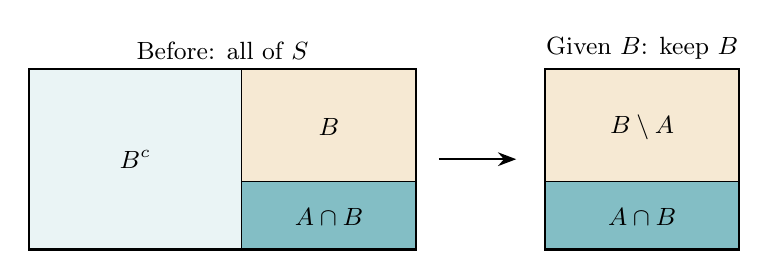
\begin{tikzpicture}[x=0.82cm,y=0.82cm,every node/.style={font=\small}]
\fill[pale] (0,0) rectangle (6,2.8);
\fill[gold!22] (3.3,0) rectangle (6,2.8);
\fill[teal!50] (3.3,0) rectangle (6,1.05);
\draw[thick] (0,0) rectangle (6,2.8);
\draw (3.3,0)--(3.3,2.8);
\draw (3.3,1.05)--(6,1.05);
\node at (1.65,1.4) {$B^c$};
\node at (4.65,1.9) {$B$};
\node at (4.65,0.5) {$A\cap B$};
\node[above] at (3,2.8) {Before: all of $S$};
\draw[-{Stealth},thick] (6.35,1.4)--(7.55,1.4);
\fill[gold!22] (8,0) rectangle (11,2.8);
\fill[teal!50] (8,0) rectangle (11,1.05);
\draw[thick] (8,0) rectangle (11,2.8);
\draw (8,1.05)--(11,1.05);
\node at (9.5,1.9) {$B\setminus A$};
\node at (9.5,0.5) {$A\cap B$};
\node[above] at (9.5,2.8) {Given $B$: keep $B$};
\end{tikzpicture}
\end{center}
Here area represents probability, and $B\setminus A$ means the part of $B$ outside $A$. The shaded fraction \emph{inside the retained group} is $\Pp(A\mid B)$.

\minihead{A quick count, when outcomes are equally likely}
Toss a fair coin independently three times. Let $A$ mean at least two heads and $B$ mean first toss heads. Of the eight equally likely outcomes, four are in $A$. Given $B$, only
\[
\underbrace{HHH,\ HHT,\ HTH}_{\text{also in }A},\ HTT
\]
remain. Thus $\Pp(A)=4/8=1/2$ but $\Pp(A\mid B)=3/4$. Counting favorable outcomes divided by total outcomes works here because the retained outcomes are equally likely.

\takeaway{$\Pp(A\mid B)$ and $\Pp(B\mid A)$ use different reference groups. Reversing the letters usually changes the answer.}

\newpage
\sectionpage{02 / MULTIPLICATION AND TOTAL PROBABILITY}{Multiply along a route; add across routes}
Rearranging the definition of conditional probability gives the \textbf{multiplication rule}:
\[
\underbrace{\Pp(A\cap B)}_{\text{both occur}}
=\underbrace{\Pp(A)}_{\text{reach }A}
\underbrace{\Pp(B\mid A)}_{\text{then satisfy }B\text{ within }A}.
\]
This identity requires $\Pp(A)>0$ when written using $\Pp(B\mid A)$. It does not require independence.

\minihead{Two aces without replacement}
Let $A_1$ mean first card is an ace and $A_2$ mean second card is an ace. After the first ace, $3$ aces remain among $51$ cards:
\[
\Pp(A_1\cap A_2)=\frac4{52}\cdot\frac3{51}=\frac1{221}.
\]
For three events, apply the same rule again:
\[
\Pp(A\cap B\cap C)=\Pp(A)\Pp(B\mid A)\Pp(C\mid A\cap B).
\]
The conditioning records \emph{everything already required} along that route. The displayed conditionals require positive conditioning probabilities. For four aces, the rule gives
$\frac4{52}\frac3{51}\frac2{50}\frac1{49}=\frac1{270725}$.

\minihead{A partition lists all mutually exclusive routes}
Events $B_1,\ldots,B_m$ partition $S$ if they do not overlap and together cover $S$. Every occurrence of an event $E$ then lies in exactly one of
\[
E\cap B_1,\ E\cap B_2,\ \ldots,\ E\cap B_m.
\]
Add these disjoint pieces, then use the multiplication rule on each:
\[
\boxed{\Pp(E)=\sum_{i=1}^{m}\Pp(E\cap B_i)
=\sum_{i=1}^{m}\Pp(E\mid B_i)\Pp(B_i).}
\]
This is the \textbf{law of total probability}. The sum symbol $\sum$ means to add one term for each index $i$. Omit any partition piece with probability zero when writing the conditional terms.

For the two routes $B$ and $B^c$, assuming both have positive probability,
\[
\Pp(E)=\underbrace{\Pp(E\mid B)\Pp(B)}_{\text{part of }E\text{ in }B}
+\underbrace{\Pp(E\mid B^c)\Pp(B^c)}_{\text{part of }E\text{ outside }B}.
\]
In the card example, the second card can be an ace whether the first was an ace or not:
\[
\Pp(A_2)=\frac3{51}\frac4{52}+\frac4{51}\frac{48}{52}=\frac4{52}.
\]
The \emph{unconditional} probability of a second ace is $4/52$, even though the \emph{conditional} probability after seeing a first ace is $3/51$.

\takeaway{A tree organizes the routes. Its later branch probabilities are conditional probabilities; drawing a tree does not make the events independent.}

\newpage
\sectionpage{03 / INDEPENDENCE}{The proportion stays the same}
Events $A$ and $B$ are \textbf{independent} exactly when
\[
\boxed{\Pp(A\cap B)=\Pp(A)\Pp(B).}
\]
If $\Pp(B)>0$, divide by $\Pp(B)$ to obtain
\[
\Pp(A\mid B)=\frac{\Pp(A)\Pp(B)}{\Pp(B)}=\Pp(A).
\]
Thus knowing $B$ occurred does not change the probability of $A$. Likewise, when $\Pp(A)>0$, independence is equivalent to $\Pp(B\mid A)=\Pp(B)$. The product definition also covers events of probability zero.

\minihead{A square in which area represents probability}
Write $a=\Pp(A)$ and $b=\Pp(B)$. In this model, $A$ is a vertical strip of width $a$ and $B$ is a horizontal strip of height $b$ in a unit square.
\begin{center}
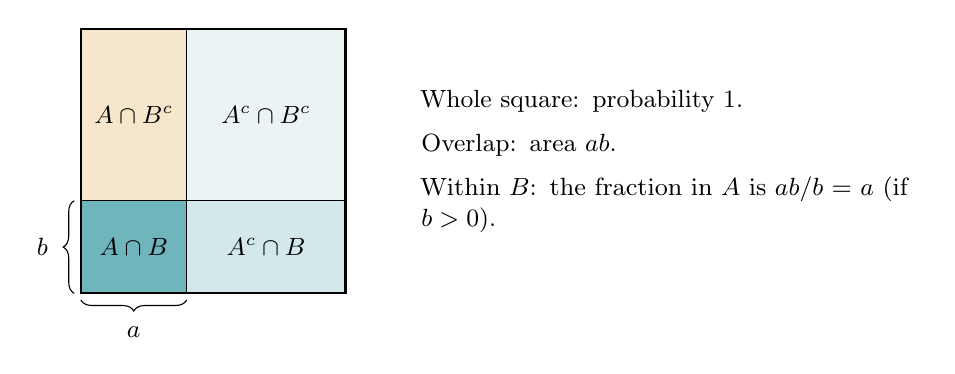
\begin{tikzpicture}[x=0.84cm,y=0.84cm,every node/.style={font=\small}]
\fill[pale] (0,0) rectangle (4,4);
\fill[gold!25] (0,0) rectangle (1.6,4);
\fill[teal!18] (0,0) rectangle (4,1.4);
\fill[teal!58] (0,0) rectangle (1.6,1.4);
\draw[thick] (0,0) rectangle (4,4);
\draw (1.6,0)--(1.6,4);\draw (0,1.4)--(4,1.4);
\node at (0.8,0.7) {$A\cap B$};
\node at (0.8,2.7) {$A\cap B^c$};
\node at (2.8,0.7) {$A^c\cap B$};
\node at (2.8,2.7) {$A^c\cap B^c$};
\draw[decorate,decoration={brace,mirror,amplitude=4pt}] (0,-0.1)--node[below=6pt]{$a$}(1.6,-0.1);
\draw[decorate,decoration={brace,amplitude=4pt}] (-0.1,0)--node[left=6pt]{$b$}(-0.1,1.4);
\node[align=left,text width=6.3cm,anchor=west] at (5,2)
{Whole square: probability $1$.\\[5pt]
Overlap: area $ab$.\\[5pt]
Within $B$: the fraction in $A$ is $ab/b=a$ (if $b>0$).};
\end{tikzpicture}
\end{center}
The diagram represents independence because the fraction in $A$ stays the same across the horizontal slices. Merely drawing perpendicular strips is not evidence that two real events are independent; the probability model must justify the product rule.

\minihead{Check the joint probability against the product}
In the course's tuition survey, $A$ means ``tuition is too high'' and $D$ means ``has a child in college.'' The table gives
\[
\Pp(A\cap D)=.35,\qquad\Pp(A)=.60,\qquad\Pp(D)=.44.
\]
Since $.35\ne .60(.44)=.264$, the events are dependent. Equivalently, $\Pp(A\mid D)=.35/.44\approx .795\ne .60$.

\takeaway{Disjoint positive-probability events are dependent: their intersection has probability $0$, while the product of their probabilities is positive. Independence allows overlap.}

\textbf{Sampling.} Uniform, independently randomized draws with replacement are independent. Without replacement, the first draw can change the composition. For a population split evenly into two groups, the chance that both draws belong to one specified group is $\frac12\frac13$ for $4$ people and $\frac12\frac{499}{999}$ for $1000$ people. The latter is close to, but different from, $1/4$.

\newpage
\sectionpage{04 / SEVERAL EVENTS}{Pairwise and mutual independence}
For three events, \textbf{pairwise independence} means that each of the three pairs is independent. \textbf{Mutual independence} requires those three identities \emph{and} the identity for the triple:
\begin{align*}
\Pp(A\cap B)&=\Pp(A)\Pp(B), & \Pp(A\cap C)&=\Pp(A)\Pp(C),\\
\Pp(B\cap C)&=\Pp(B)\Pp(C), & \Pp(A\cap B\cap C)&=\Pp(A)\Pp(B)\Pp(C).
\end{align*}
Checking only the pairs is insufficient. Checking only the triple is also insufficient.

\minihead{Why pairwise independence is not enough}
Choose uniformly from $S=\{1,2,3,4\}$, and define
\[
A=\{1,4\},\qquad B=\{2,4\},\qquad C=\{3,4\}.
\]
\begin{center}
\begin{tabular}{@{}ccccc@{}}\toprule
Outcome & 1 & 2 & 3 & 4\\\midrule
In $A$? & yes & no & no & yes\\
In $B$? & no & yes & no & yes\\
In $C$? & no & no & yes & yes\\\bottomrule
\end{tabular}
\end{center}
Each event has probability $1/2$. Every pair intersects at just $\{4\}$, so every pair has intersection probability $1/4=(1/2)(1/2)$. But the triple also intersects at $\{4\}$:
\[
\Pp(A\cap B\cap C)=\frac14\ne\frac18=\Pp(A)\Pp(B)\Pp(C).
\]
These events are pairwise independent but not mutually independent. Knowing $A$ alone leaves $\Pp(C\mid A)=1/2$. Knowing \emph{both} $A$ and $B$ forces the outcome to be $4$, giving $\Pp(C\mid A\cap B)=1$.

\minihead{The general definition}
Events $A_1,\ldots,A_n$ are mutually independent when \emph{every selection of two or more events} has intersection probability equal to the product of its individual probabilities. In compact notation,
\[
\Pp\!\left(\bigcap_{i\in I}A_i\right)=\prod_{i\in I}\Pp(A_i)
\quad\text{for every index set }I\text{ with at least two members}.
\]
The large intersection symbol means ``all of the selected events occur''; the product symbol means ``multiply the selected probabilities.''

\minihead{Complements preserve independence}
If $A$ and $B$ are independent, then
\begin{align*}
\Pp(A\cap B^c)
&=\Pp(A)-\Pp(A\cap B) &&\text{remove the part inside }B\\
&=\Pp(A)-\Pp(A)\Pp(B) &&\text{use independence}\\
&=\Pp(A)\Pp(B^c). &&\text{factor and use }1-\Pp(B)
\end{align*}
So $A$ and $B^c$ are also independent. For mutually independent events, an event is independent of combinations of the other events using unions, intersections, and complements. For example,
$\Pp(A\mid B^c\cap C)=\Pp(A)$ when the conditioning event has positive probability.

\newpage
\sectionpage{05 / BAYES' FORMULA}{One overlap, two reference groups}
Suppose $B$ represents a possible source or explanation, and $E$ represents observed evidence. We may know $\Pp(E\mid B)$ but want $\Pp(B\mid E)$.

Write the probability of their overlap in two ways:
\[
\Pp(B\cap E)=\Pp(E\mid B)\Pp(B)=\Pp(B\mid E)\Pp(E).
\]
Dividing by $\Pp(E)$ gives \textbf{Bayes' formula}:
\[
\boxed{\underbrace{\Pp(B\mid E)}_{\text{posterior}}
=\frac{\underbrace{\Pp(E\mid B)}_{\text{likelihood}}\,
\underbrace{\Pp(B)}_{\text{prior}}}{\underbrace{\Pp(E)}_{\text{total probability of evidence}}}.}
\]
Here $\Pp(B)>0$ and $\Pp(E)>0$ so the displayed conditionals are defined.
\begin{itemize}
\item The \textbf{prior} is the probability assigned to $B$ before incorporating $E$.
\item The \textbf{likelihood} is how probable $E$ is if $B$ holds.
\item The \textbf{posterior} is the probability assigned to $B$ after incorporating $E$.
\end{itemize}
The likelihood and posterior ask different questions. Their numerators can describe the same overlap, but their reference groups differ.

\minihead{See the denominator as all the observed evidence}
Let $b=\Pp(B)$, $u=\Pp(E\mid B)$, and $v=\Pp(E\mid B^c)$, with $0<b<1$. In the unit-area diagram, the widths represent the prior probabilities and the shaded heights represent the two likelihoods.
\begin{center}
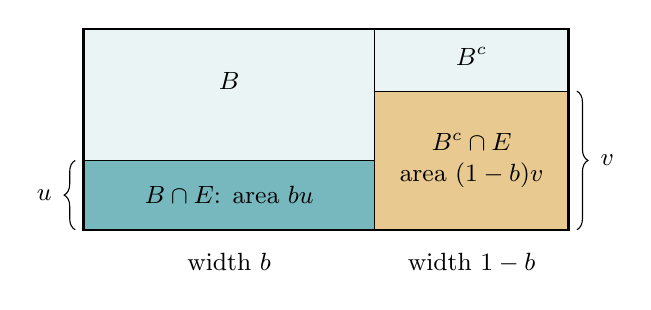
\begin{tikzpicture}[x=0.88cm,y=0.88cm,every node/.style={font=\small}]
\fill[pale] (0,0) rectangle (7,2.9);
\fill[teal!55] (0,0) rectangle (4.2,1.0);
\fill[gold!55] (4.2,0) rectangle (7,2.0);
\draw[thick] (0,0) rectangle (7,2.9);
\draw (4.2,0)--(4.2,2.9);
\draw (0,1)--(4.2,1);\draw (4.2,2)--(7,2);
\node at (2.1,2.15) {$B$};\node at (5.6,2.5) {$B^c$};
\node at (2.1,0.5) {$B\cap E$: area $bu$};
\node[align=center] at (5.6,1) {$B^c\cap E$\\area $(1-b)v$};
\node[below=5pt] at (2.1,0) {width $b$};
\node[below=5pt] at (5.6,0) {width $1-b$};
\draw[decorate,decoration={brace,amplitude=4pt}] (-0.12,0)--node[left=5pt]{$u$}(-0.12,1);
\draw[decorate,decoration={brace,mirror,amplitude=4pt}] (7.12,0)--node[right=5pt]{$v$}(7.12,2);
\end{tikzpicture}
\end{center}
After observing $E$, retain both shaded pieces. The fraction of their combined area coming from $B$ is
\[
\Pp(B\mid E)=\frac{bu}{bu+(1-b)v}
=\frac{\Pp(E\mid B)\Pp(B)}{\Pp(E\mid B)\Pp(B)+\Pp(E\mid B^c)\Pp(B^c)}.
\]
\takeaway{Bayes' formula keeps the overlap in the numerator and divides by the total probability of the evidence. Include every route that could have produced the evidence.}

\newpage
\sectionpage{06 / BAYESIAN UPDATING}{Weight the alternatives, then normalize}
Let $B_1,\ldots,B_m$ be a partition into possible alternatives with positive probability. For evidence $E$ with $\Pp(E)>0$, define the weights
\[
w_i=\underbrace{\Pp(B_i)}_{\text{prior}}\underbrace{\Pp(E\mid B_i)}_{\text{likelihood}}
=\Pp(B_i\cap E).
\]
The weights sum to $\Pp(E)$ by total probability. Dividing each weight by that sum makes the resulting probabilities add to $1$:
\[
\boxed{\Pp(B_i\mid E)=\frac{w_i}{w_1+\cdots+w_m}
=\frac{\Pp(E\mid B_i)\Pp(B_i)}{\sum_{j=1}^{m}\Pp(E\mid B_j)\Pp(B_j)}.}
\]
This final division is called \textbf{normalization}.

\minihead{Worked example: the three urns from class}
A fair die selects an urn: rolls $1$--$3$ select urn 1, roll $4$ selects urn 2, and rolls $5$--$6$ select urn 3. Draw a marble uniformly from the selected urn. Let $B_i$ mean urn $i$ was selected and $R$ mean a red marble was drawn.
\begin{center}
\renewcommand{\arraystretch}{1.3}
\begin{tabular}{@{}lcccc@{}}\toprule
& Contents & Prior & Likelihood & Weight\\
& & $\Pp(B_i)$ & $\Pp(R\mid B_i)$ & $\Pp(B_i\cap R)$\\\midrule
Urn 1 & 5 white, 1 red & $1/2$ & $1/6$ & $1/12$\\
Urn 2 & 0 white, 7 red & $1/6$ & $1$ & $1/6$\\
Urn 3 & 3 white, 3 red & $1/3$ & $1/2$ & $1/6$\\\bottomrule
\end{tabular}
\end{center}
Add the weights to find $\Pp(R)=1/12+1/6+1/6=5/12$. Then
\[
\Pp(B_2\mid R)=\frac{1/6}{5/12}=\frac25.
\]
The full update is
\[
\underbrace{(1/2,\ 1/6,\ 1/3)}_{\text{prior urn probabilities}}
\quad\longrightarrow\quad
\underbrace{(1/5,\ 2/5,\ 2/5)}_{\text{posterior urn probabilities given red}}.
\]
Urn 2's prior was only $1/6$, but red is certain under urn 2. The evidence increases its probability to $2/5$. Urn 1 becomes less probable because red is comparatively unlikely under urn 1.

\minihead{Update again when new evidence arrives}
The posterior after one observation can serve as the prior for the next. If the first evidence is $E_1$ and the new evidence is $E_2$, then
\[
\Pp(B_i\mid E_1\cap E_2)=
\frac{\Pp(E_2\mid B_i\cap E_1)\Pp(B_i\mid E_1)}
{\sum_j\Pp(E_2\mid B_j\cap E_1)\Pp(B_j\mid E_1)}.
\]
Assume $\Pp(E_1\cap E_2)>0$ and omit alternatives with $\Pp(B_j\cap E_1)=0$. The new likelihood must reflect the first observation. It simplifies to $\Pp(E_2\mid B_i)$ only when $E_1$ and $E_2$ are conditionally independent given $B_i$.

\newpage
\sectionpage{07 / INTERPRETATION AND PRACTICE}{Use the formulas to explain what changes}
\minihead{A probability and an observed frequency are different quantities}
For repeated independent trials in which an event $E$ has the same probability $p$, define
\[
f_n(E)=\frac{\text{number of times }E\text{ occurs in the first }n\text{ trials}}{n}.
\]
The law of large numbers says that $f_n(E)$ converges to $p$ with probability $1$. A finite frequency estimates $p$; it need not equal $p$ or move closer at every new trial. A run of heads does not make tails ``due'' on the next independent fair toss.

Historical frequencies describe the population and conditions that produced them. Using one to predict a new outcome requires a probability model and assumptions about comparability. Bayesian updating also uses a probability model: it changes probabilities assigned to hypotheses or unknown quantities after evidence arrives.

\minihead{Independence is stronger than zero correlation}
For random variables with finite second moments, independence implies zero covariance. When both variances are positive, it also implies zero correlation. The converse is false: zero correlation does not rule out nonlinear dependence. Approximate equality of proportions in a finite data set is likewise not a proof of independence.

\minihead{Try these before reading the answers}
\begin{enumerate}[itemsep=5pt]
\item In $\Pp(A\mid B)$, which event determines the denominator, and why?
\item If $\Pp(A)=.4$, $\Pp(B)=.5$, and $\Pp(A\cap B)=.2$, are $A$ and $B$ independent? What is $\Pp(A\mid B)$?
\item Can two disjoint events with positive probability be independent?
\item For three events, why is checking all three pairs insufficient?
\item In the urn example, why is the Bayes denominator $5/12$ rather than $1/6$? If the marble is white, find $\Pp(B_1\mid W)$.
\item Must a sequence of observed heads proportions get closer to $1/2$ at every toss?
\end{enumerate}

\minihead{Answers and reasoning}
\begin{enumerate}[itemsep=5pt]
\item $B$: we restrict the reference group to outcomes in $B$, so divide the overlap's probability by $\Pp(B)$.
\item Yes: $.2=.4(.5)$. Also $\Pp(A\mid B)=.2/.5=.4$, equal to $\Pp(A)$.
\item No: their intersection probability is zero but the product is positive.
\item The probability of the triple intersection must also factor. Section 4 gives a case in which every pair factors but the triple does not.
\item $5/12$ counts \emph{all} red paths; $1/6$ counts only the red path through urn 2. For white, $\Pp(W)=1-5/12=7/12$, so
$\Pp(B_1\mid W)=\frac{(5/6)(1/2)}{7/12}=5/7$.
\item No. Convergence describes long-run behavior, not a monotone approach.
\end{enumerate}

\vfill
{\footnotesize\textbf{Course connection.} Prepared from the Chapter 4 course notes and the September 21 lecture guide for EN.553.211, Probability and Statistics for the Life Sciences. The geometric explanations, notation guide, and worked calculations supplement the course material.}
\end{document}
